\tikzset{every picture/.style={line width=0.75pt}} %set default line width to 0.75pt        

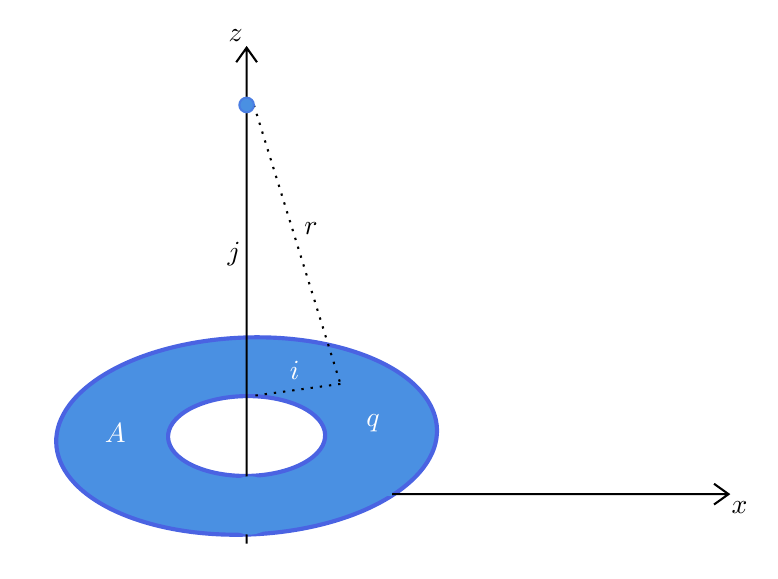
\begin{tikzpicture}[x=0.75pt,y=0.75pt,yscale=-1,xscale=1]
%uncomment if require: \path (0,430); %set diagram left start at 0, and has height of 430

%Shape: Donut [id:dp7549476977820966] 
\draw  [color={rgb, 255:red, 74; green, 99; blue, 226 }  ,draw opacity=1 ][fill={rgb, 255:red, 74; green, 144; blue, 226 }  ,fill opacity=1 ,even odd rule][line width=1.5]  (194.66,267.55) .. controls (176.97,262.03) and (171.64,250.2) .. (182.76,241.12) .. controls (193.88,232.03) and (217.24,229.14) .. (234.94,234.65) .. controls (252.63,240.17) and (257.96,252) .. (246.84,261.08) .. controls (235.72,270.17) and (212.36,273.06) .. (194.66,267.55)(164.46,292.22) .. controls (122.11,279.03) and (110.32,249.92) .. (138.13,227.21) .. controls (165.93,204.51) and (222.8,196.79) .. (265.14,209.98) .. controls (307.49,223.17) and (319.28,252.28) .. (291.47,274.99) .. controls (263.67,297.69) and (206.8,305.41) .. (164.46,292.22) ;
%Shape: Axis 2D [id:dp24379060919610995] 
\draw  (189,279.1) -- (447,279.1)(214.8,64) -- (214.8,303) (440,274.1) -- (447,279.1) -- (440,284.1) (209.8,71) -- (214.8,64) -- (219.8,71)  ;
%Shape: Circle [id:dp6435227629373832] 
\draw  [color={rgb, 255:red, 74; green, 144; blue, 226 }  ,draw opacity=1 ][fill={rgb, 255:red, 74; green, 144; blue, 226 }  ,fill opacity=1 ] (202.8,284.55) .. controls (202.8,277.07) and (208.87,271) .. (216.35,271) .. controls (223.83,271) and (229.9,277.07) .. (229.9,284.55) .. controls (229.9,292.03) and (223.83,298.1) .. (216.35,298.1) .. controls (208.87,298.1) and (202.8,292.03) .. (202.8,284.55) -- cycle ;
%Straight Lines [id:da35931985921212983] 
\draw [color={rgb, 255:red, 74; green, 144; blue, 226 }  ,draw opacity=1 ][fill={rgb, 255:red, 255; green, 255; blue, 255 }  ,fill opacity=1 ][line width=1.5]    (253,279) -- (285,279) ;
%Straight Lines [id:da44873433810971197] 
\draw [color={rgb, 255:red, 74; green, 144; blue, 226 }  ,draw opacity=1 ][line width=1.5]    (187,279) -- (253,279) ;
%Straight Lines [id:da19987966215329656] 
\draw  [dash pattern={on 0.84pt off 2.51pt}]  (218.3,91.6) -- (260,226) ;
%Shape: Circle [id:dp9633618470790888] 
\draw  [color={rgb, 255:red, 74; green, 125; blue, 226 }  ,draw opacity=1 ][fill={rgb, 255:red, 74; green, 144; blue, 226 }  ,fill opacity=1 ] (211.3,91.6) .. controls (211.3,89.67) and (212.87,88.1) .. (214.8,88.1) .. controls (216.73,88.1) and (218.3,89.67) .. (218.3,91.6) .. controls (218.3,93.53) and (216.73,95.1) .. (214.8,95.1) .. controls (212.87,95.1) and (211.3,93.53) .. (211.3,91.6) -- cycle ;
%Straight Lines [id:da26890877688664827] 
\draw  [dash pattern={on 0.84pt off 2.51pt}]  (260,226) -- (216,232) ;
%Straight Lines [id:da09923872552730995] 
\draw [draw opacity=0]   (214.8,95.1) -- (216,232) ;

% Text Node
\draw (145,243.4) node [anchor=north west][inner sep=0.75pt]  [color={rgb, 255:red, 255; green, 255; blue, 255 }  ,opacity=1 ]  {$A$};
% Text Node
\draw (271,239.4) node [anchor=north west][inner sep=0.75pt]  [color={rgb, 255:red, 255; green, 255; blue, 255 }  ,opacity=1 ]  {$q$};
% Text Node
\draw (213.4,163.55) node [anchor=east] [inner sep=0.75pt]    {$j$};
% Text Node
\draw (241.15,155.4) node [anchor=south west] [inner sep=0.75pt]    {$r$};
% Text Node
\draw (238,225.6) node [anchor=south] [inner sep=0.75pt]  [color={rgb, 255:red, 255; green, 255; blue, 255 }  ,opacity=1 ]  {$i$};
% Text Node
\draw (214.44,62.6) node [anchor=south east] [inner sep=0.75pt]    {$z$};
% Text Node
\draw (447,281.4) node [anchor=north west][inner sep=0.75pt]    {$x$};

\end{tikzpicture}
